\documentclass{ime-beamer}
\usepackage[portuges]{babel}
\usepackage[utf8]{inputenc}
\usepackage{graphicx}
\usepackage[portuguese]{algorithm2e}% Para escrever algorítimos
\usepackage{listings}			% Para usar \lstinputlisting e incluir código
\usepackage{subcaption}			% Para usar \begin{subfigure} e colocar figuras (a) e (b) lado a lado

\title[Técnicas de IA aplicadas ao futebol de robôs]{%
  Técnicas de IA Aplicadas a Sistemas Multiagentes Cooperativos e Competitivos
}
\author[Jan Segre\and Victor Bramigk]{%
  Jan Segre\\
  Victor Bramigk\\
  Paulo F. F. Rosa (Orientador)\\
  Bruno Madeira (Co-orientador)
}

% as imagens ficam nesse diretório
\graphicspath{{img/}}

\begin{document}
\frame{\maketitle}

\frame{%
  \frametitle{Roteiro}
  \tableofcontents
}

\section{Introdução}
\frame{%
  \frametitle{Robocup}
  \begin{block}{}
    \begin{figure}
      \centering
      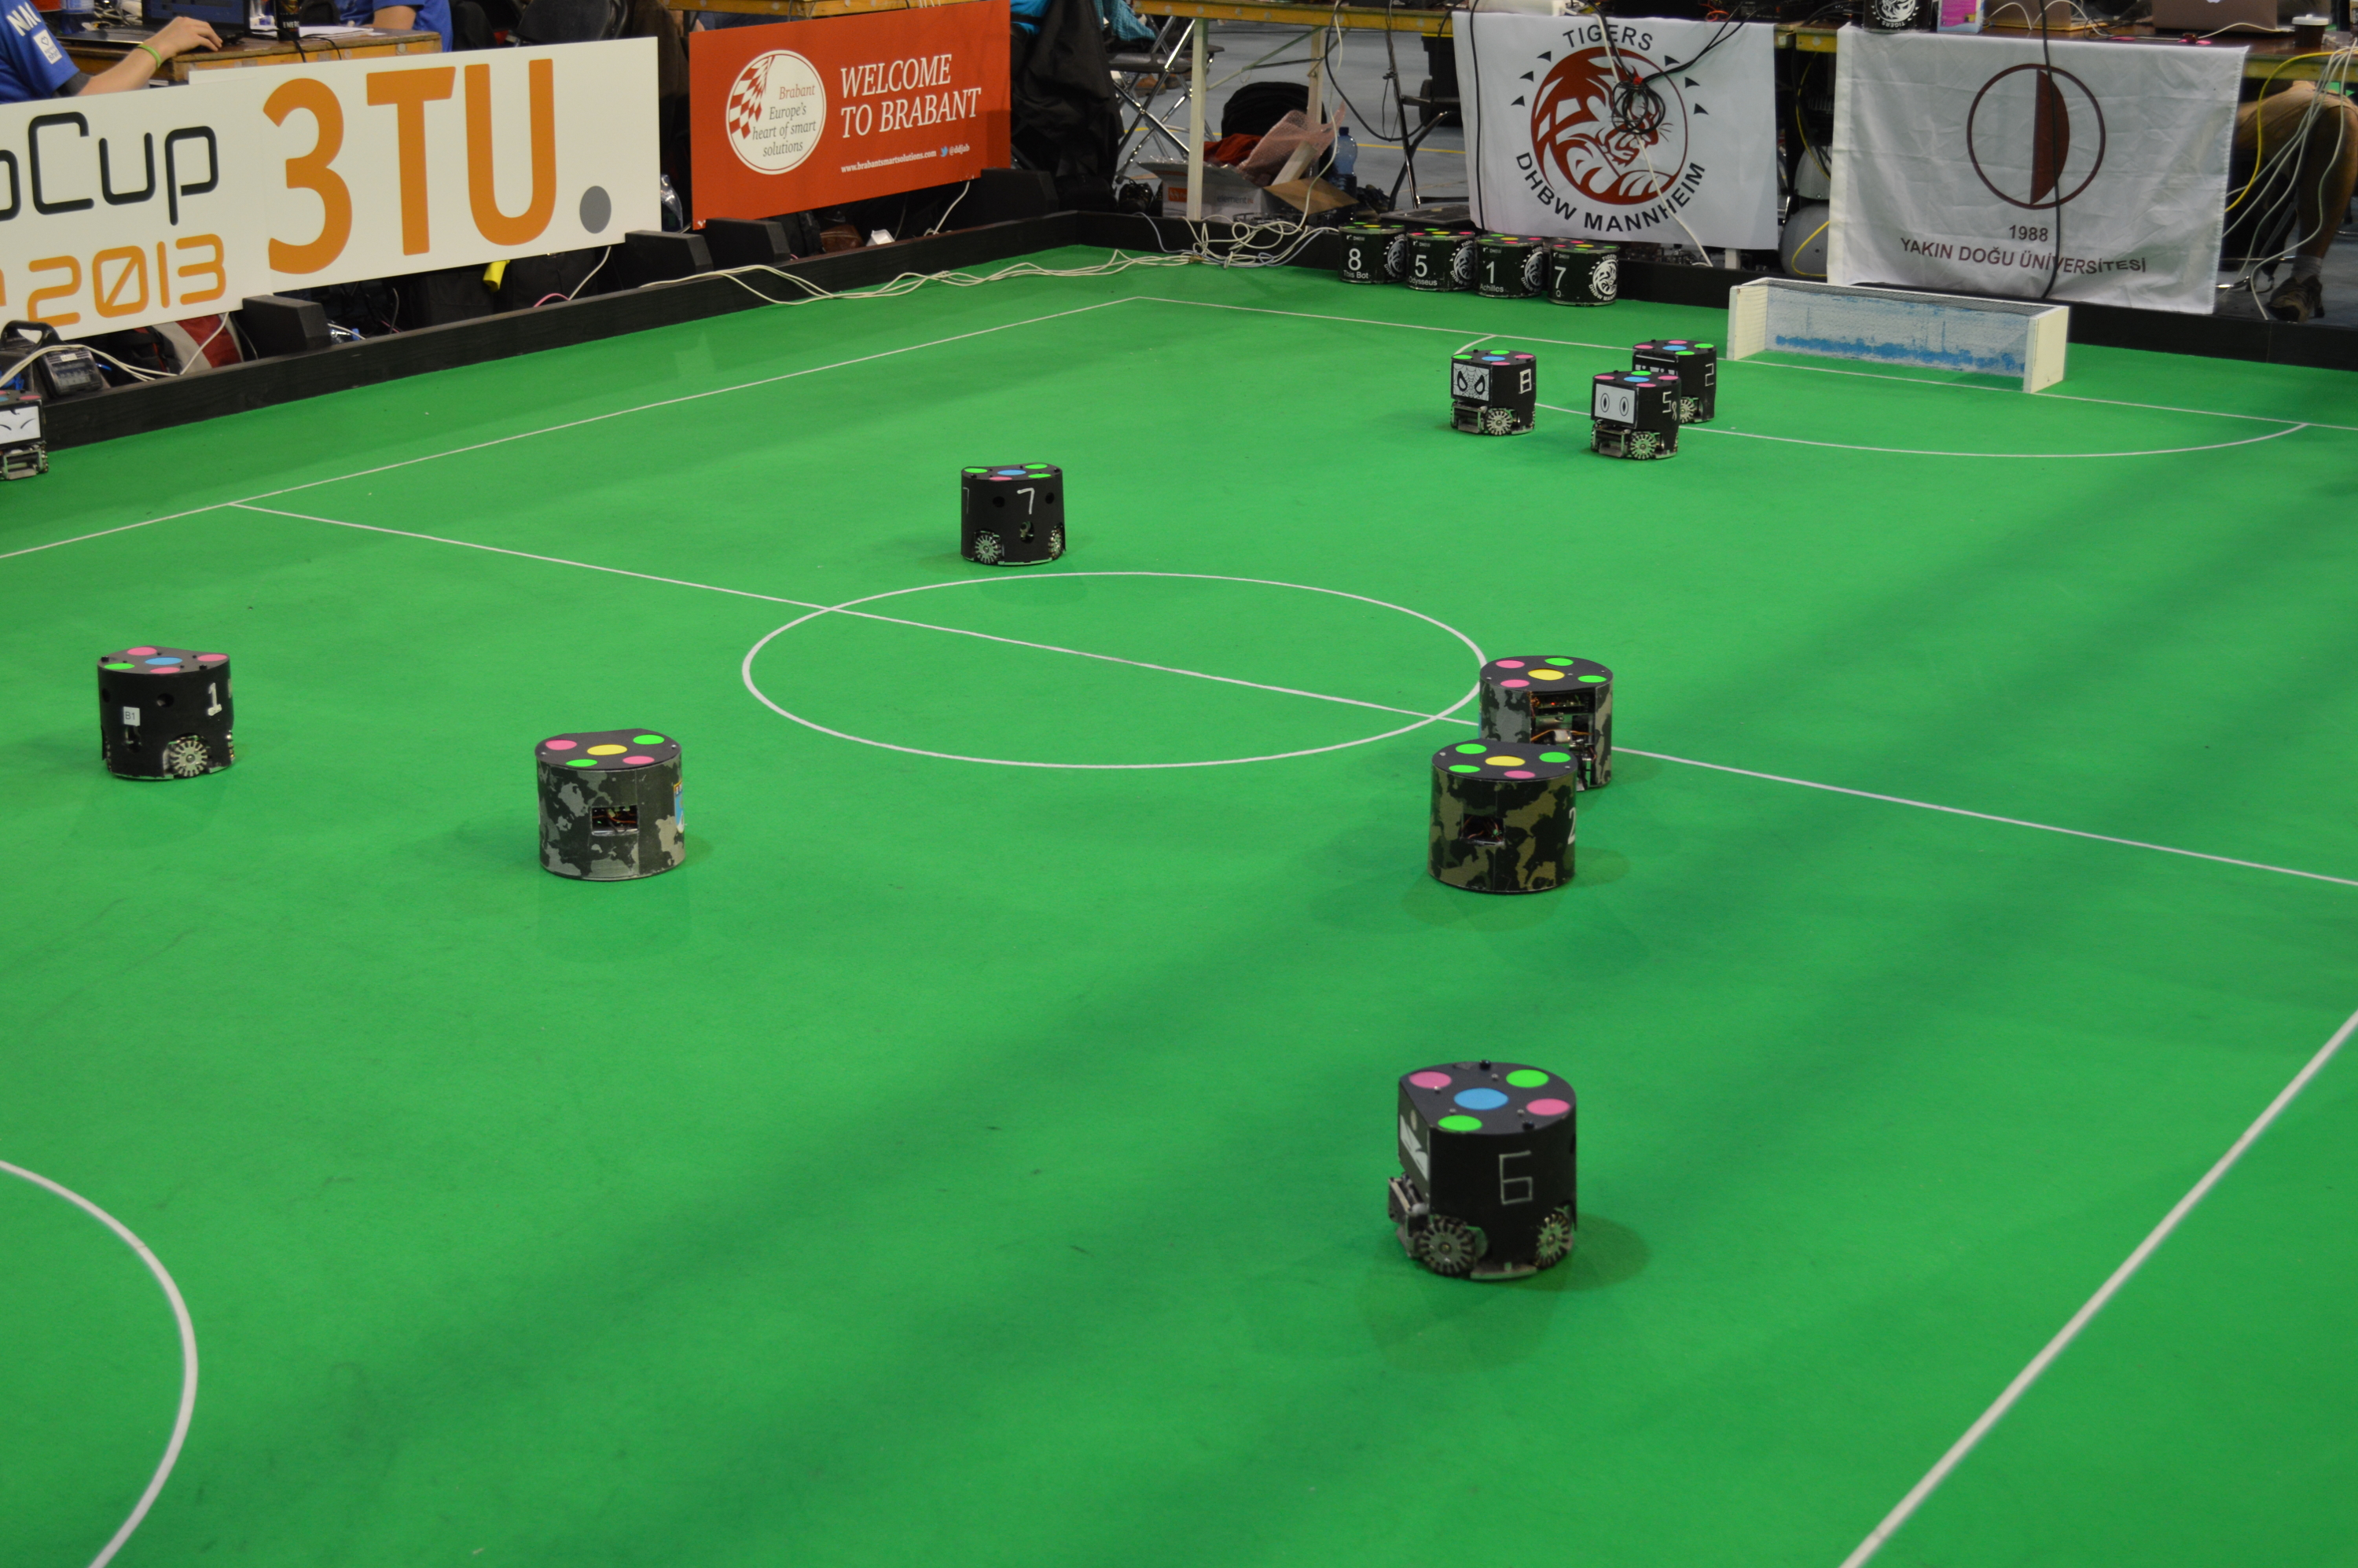
\includegraphics[width=0.7\linewidth]{robocup2013}
      \caption{Imagem da SSL \textit{RoboCup} 2013 em Eindhoven, na Holanda}\label{fig:robocup2013}
    \end{figure}
  \end{block}
}

\section{Minimax}
\frame{%
  \frametitle{Minimax}
  \begin{block}{}
    \centering
    Regra de decisão para minimizar a perda máxima.

    Se aplica a um jogo $\Gamma=\langle A,B,H\rangle$ quando:

    \begin{gather}
      v=\max_{a\in A}\min_{b\in B}H(a,b)=\min_{b\in B}\max_{a\in A}H(a,b)\label{eq:req}
    \end{gather}
  \end{block}
}
\frame{%
  \frametitle{Minimax}
  \begin{block}{}
    \begin{figure}[H]
      \centering
      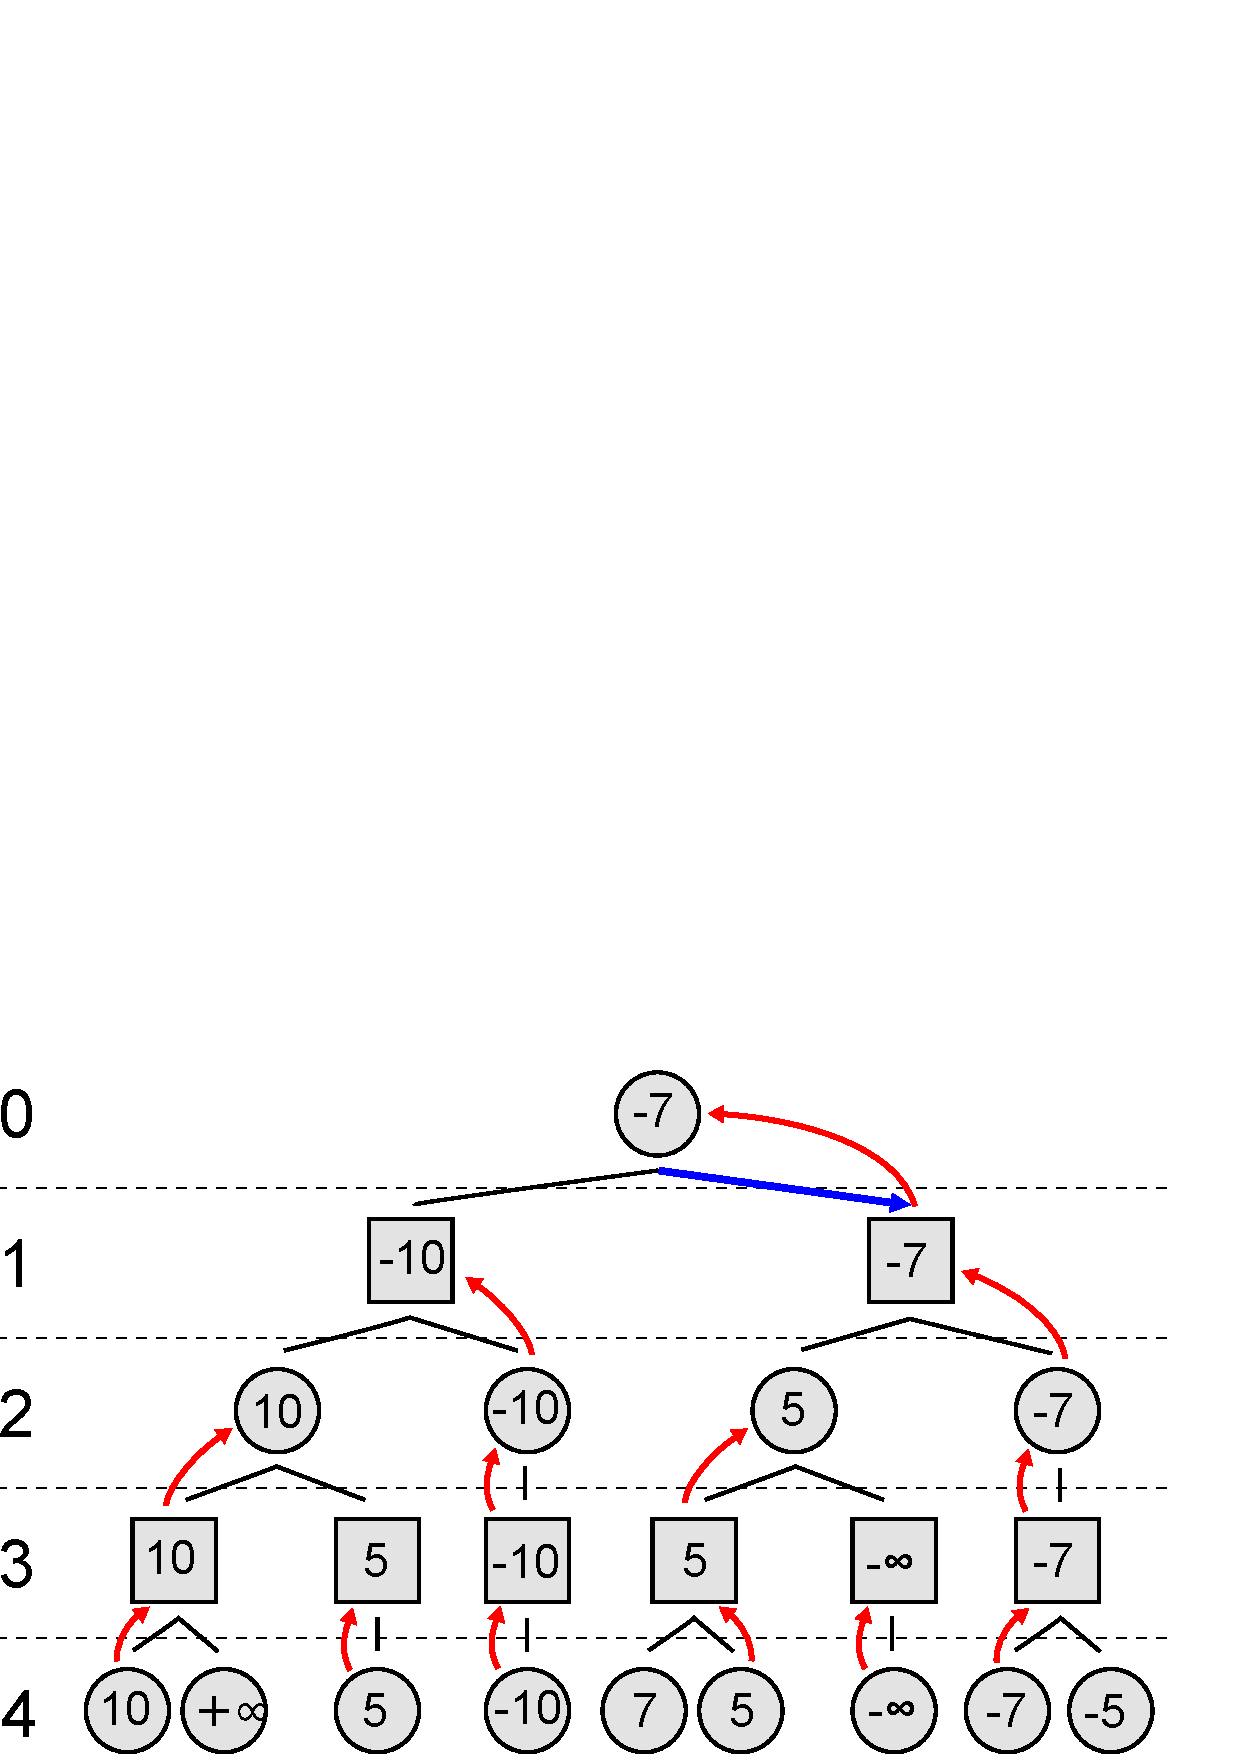
\includegraphics[width=0.7\linewidth]{minimax-tree}
      \caption{Exemplo de árvore de decisão com Minimax.}\label{fig:minimax-tree}
    \end{figure}
  \end{block}
}

\section{Mapeamento para um jogo discreto}
\frame{%
  \frametitle{Mapeamento para um jogo discreto}
  \begin{block}{}
    \centering
    Mapear um jogo contínuo em tempo e espaço para um jogo discreto em pelo
    menos no tempo, isto é, jogadas bem definidas.
  \end{block}
}
\frame{%
  \frametitle{Mapeamento para um jogo discreto}
  \begin{block}{}
    \centering
    Mapeamento proposto:

    \begin{itemize}
      \item Ação de um time com a bola é uma lista de:
        \begin{itemize}
          \item robô sem a bola:
            \begin{itemize}
              \item $Move(x, y)$
            \end{itemize}
          \item robô com a bola:
            \begin{itemize}
              \item $Kick(x, y)$
              \item $Pass(r)$
            \end{itemize}
        \end{itemize}
      \item Ação de um time sem a bola é uma lista de:
        \begin{itemize}
          \item $Move(x, y)$
        \end{itemize}
    \end{itemize}
  \end{block}
}

\section{Experiências prévias}

\section{Cronograma}
\frame{%
  \frametitle{Cronograma}
  \begin{table}[Ht!]
    \begin{center}
      \begin{tabular}{|c|c|c|c|c|c|c|c|c|c|}
        \hline
        Data                   & Ago & Set & 0ut & Nov & Fev & Mar & Abr & Mai \\
        \hline
        \small{Modelagem do}   &  x  &  x  &     &     &     &     &     &     \\
        \small{mapeamento}     &     &     &     &     &     &     &     &     \\
        \hline
        \small{Prova de}       &     &     &  x  &  x  &     &     &     &     \\
        \small{conceito}       &     &     &     &     &     &     &     &     \\
        \hline
        \small{Implementação}  &     &     &  x  &  x  &     &     &     &     \\
        \small{da arquitetura} &     &     &     &     &     &     &     &     \\
        \hline
        \small{Implementação}  &     &     &     &     &  x  &  x  &  x  &     \\
        \small{do algoritmo}   &     &     &     &     &     &     &     &     \\
        \hline
        \small{Otimização}     &     &     &     &     &     &     &     &   x \\
        \small{do algoritimo}  &     &     &     &     &     &     &     &     \\
        \hline
      \end{tabular}
    \end{center}
  \end{table}
}

\end{document}
% vim: tw=80 et ts=2 sw=2 sts=2
